\newpage
\section{Описание разрабатываемой автоматизированной системы коммерческого учета энергоресурсов}
\setcounter{figure}{0}

Основными  потребителями  электросчетчиков российского производства являются страны СНГ, Украина и Казахстан – лидеры по потреблению в 2007-2013 году (на долю экспорта в эти страны приходится около  80\% [1] ). Для учета использования электроэнергии существуют автоматизированные системы коммерческого учета электроэнергии (АСКУЭ).

Автоматизированная система коммерческого учета энергоресурсов (АСКУЭ) - это программно-аппаратный комплекс, предназначенный для сбора, хранени и обработки инофрмации о потреблении энергоресурсов на объекте. 

Аппаратная часть представлена устройствами учета(УУ), устройствами сбора и передачи данных(УСПД), а так же центральным сервером(ЦС).

Программная часть включает в себя прошивки УУ и УСПД, ПО для ЦС.

ПО ЦС предназначено для сбора показаний с точек учета энергоресурсов, а также архивирования, хранения, анализа и визуализации полученных данных, формирования отчетов. Под показаниями подразумеваются данные о потребляемой мощности электроэнергии потребителями однофазных и трехфазных сетей.

Областью применения ПО ЦС являются объекты жилого, коммерческого и производственного назначения.

ПО ЦС — это программный комплекс, который должен включать в себя сервер баз данных, сервер сбора данных(ССД), сервер приложений, web-сервер, АРМ оператора, АРМ администратора, АРМ клиента, АРМ сервисного инженера(АРМ СИ).

ПО ССД должно выполнять следующие функции:
\begin{itemize}
 \item взаимодействие с УСПД и счетчиками (опрос и сбор данных);
 \item взаимодействие с СБД (запись обработанных данных для дальнейшей работы с ними);
 \item преобразование полученных данных в удобный для дальнейшей обработки формат;
 \item мониторинг и обработка ошибок;
 \item журналирование событий ССД.
\end{itemize}

ПО ЦС представляет собой иерархическую систему сбора, передачи и хранения данных (рис. \ref{irsh:irsh}). Информация от первичных приборов учета посредством УСПД поступает на ССД, который обеспечивает ее обработку и запись на СБД.

\begin{figure}[h!]
 \center{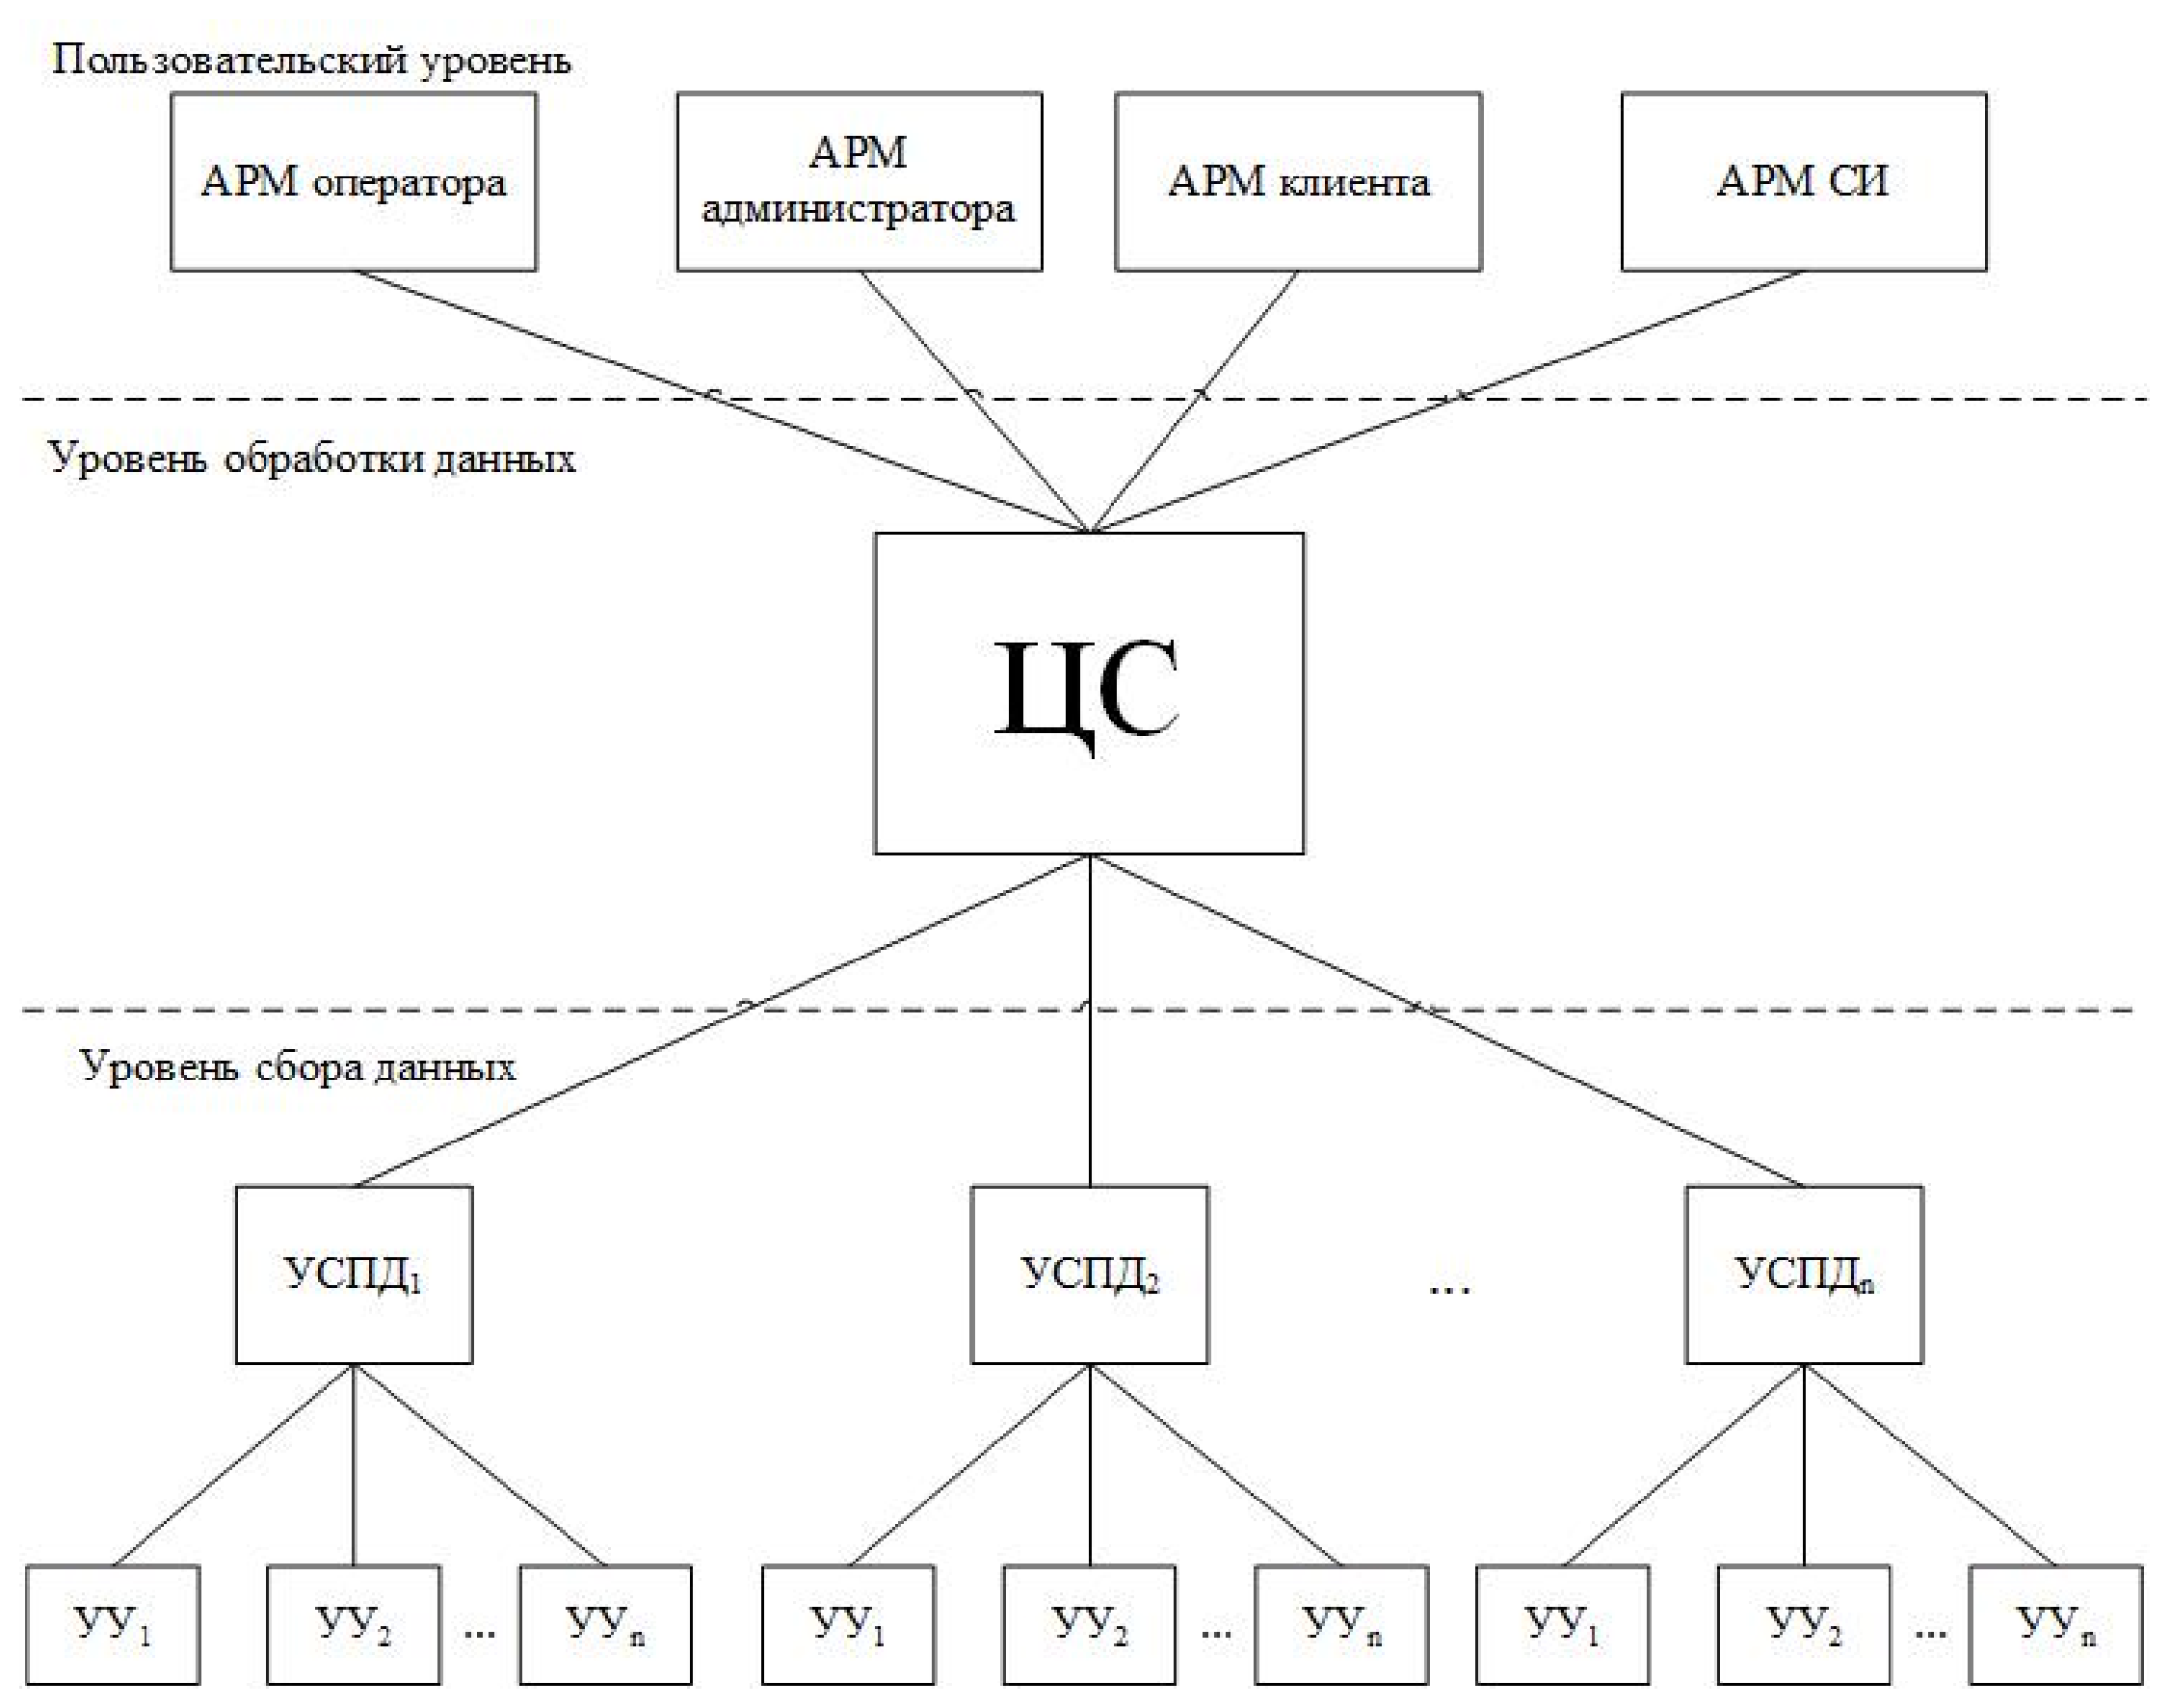
\includegraphics[width=0.8\linewidth]{irsh}}
 \caption{Структурная схема АСКУЭ}
 \label{irsh:irsh}
\end{figure}

\subsection{Описание сервера сбора данных}

ССД обслуживает низкоуровневое взаимодействие с УСПД. После получения данных этот блок передает информацию модульной системе драйверов. Система драйверов осуществляет взаимодействие на верхнем уровне модели OSI. За счет модульности обеспечивается расширение парка поддерживаемого оборудования. Также ССД содержит систему управления сетью и взаимодействия с базой данных: он осуществляет контроль работоспособности сети, выполняет отбраковку данных, отвечает за принятие решений о повторном запросе на сбор данных, классифицирует информацию, обеспечивает контроль единого времени и осуществляет запись информации в базу данных.

Логически ПО ССД можно разделить на 3 блока, каждый из которых выполняет отдельную задачу:
\begin{enumerate}
\item блок контроля приема и передачи данных, который отвечает за взаимодействие ССД с УСПД;
\item временная база данных (ВБД). В ходе проектирования ПО ССД было рассмотрено два варианта обработки и записи данных с УСПД/УУ на СБД: 
\begin{itemize}
\item обработка и запись данных на СБД по мере их поступления от УСПД;
\item запись поступающих данных в ВБД и последующая обработка и передача на СБД.
\end{itemize}
\item блок обработки данных.
\end{enumerate}

Использование первого варианта может привести к потере данных, так как вновь поступающие данные не будут успевать обрабатываться ПО ССД. Второй вариант позволяет обеспечить целостность поступивших данных, поэтому он является более предпочтительным.

Обобщенная функциональная схема функционирования ПО ССД представлена на рисунке \ref{fs_ssd:fs_ssd}.

\begin{figure}[h!]
 \center{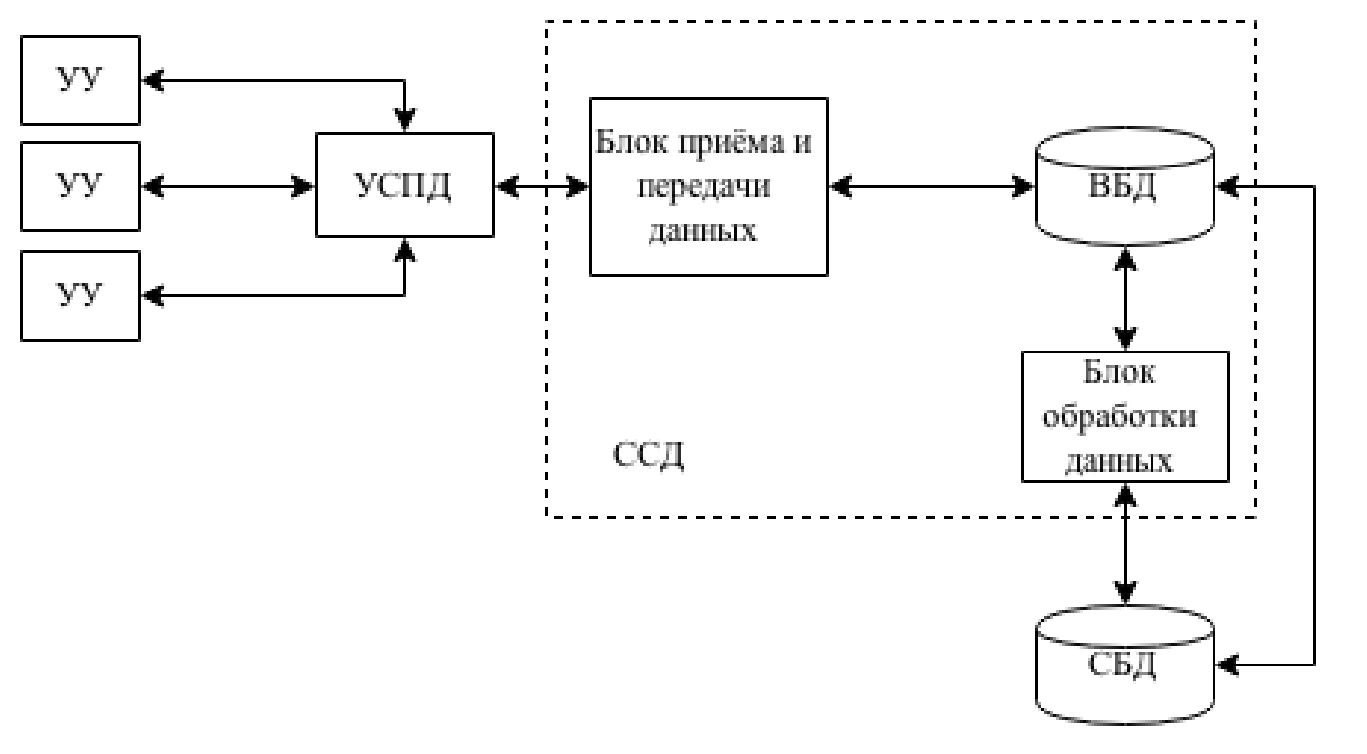
\includegraphics[width=0.8\linewidth]{fs_ssd}}
 \caption{Функциональная схема ССД}
 \label{fs_ssd:fs_ssd}
\end{figure}

Сервер сбора данных должен отвечать следующим требованиям:

\begin{itemize}
 \item работать с УСПД в количестве до 10000 устройств;
 \item передавать данные по сети интернет;
 \item контроль подключаемых устройств;
 \item контроль целостности данных;
 \item возможность добавления УСПД в запущенную систему;
 \item оперативная реакция на сигналу УСПД о неполадках.
\end{itemize}

\subsection{Описание устройства сбора и передачи данных}%TODO

Устройство сбора и передачи данных является промежуточным звеном между устройствами учета и сервером сбора данных. Оно предназначено для непосредственного управления устройствами учета, их опроса, настройки и диагностики. Всю информацию от устройств учета и о их состоянии ССД получает от УСПД.

Требования, предъявляемые к УСПД:

\begin{itemize}
 \item контроль подключений;
 \item идентификация и аутентификация пользователей;
\end{itemize}

\subsection{Взаимодействие ССД и УСПД}

Сервер сбора данных должен запрашивать с УСПД показагия всех УУ и информацию о состоянии УУ и самого УСПД. Связь устанавливается при запросе данных. Обмен данных должен начинаться с идентификации и аутентификации ССД на УСПД. После окончания сбора данных производится завершение сеанса на УСПД и разрыв соединения.

Функциональная схема данного процеса представлена на рисунке \ref{img:main_idef0}. Под алгоритмами понимаются алгоритмы опроса УСПД сервером.

\begin{figure}[!Ht]
 \center{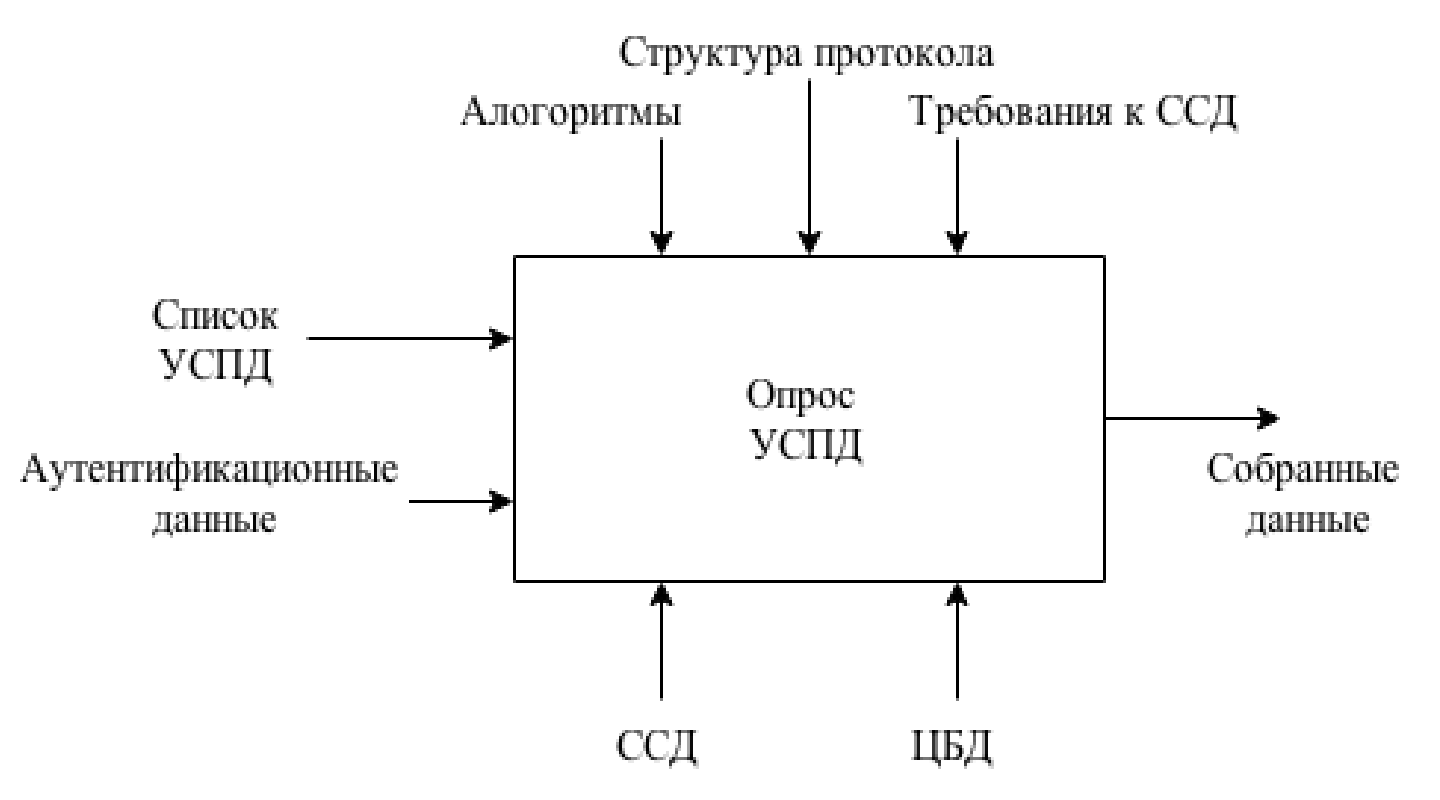
\includegraphics[width=0.8\linewidth]{main_idef0}}
 \caption{Функциональная схема процесса опроса УСПД}
 \label{img:main_idef0}
\end{figure}

После получения данных со всех УСПД происходит их обработка и отравка в центральнуб базу данных(ЦБД). В ЦБД так же хранится список всех УСПД, подконтрольных ССД.

Данные необходимо шифровать при передаче.

В разрабатываемой системе сервер является инициатором всех обменов данными, а клиенты ожидают запроса для передачи данных. Схема взаимодействия приведена на рисунке \ref{scheme2:scheme2}.

\begin{figure}[!ht]
 \center{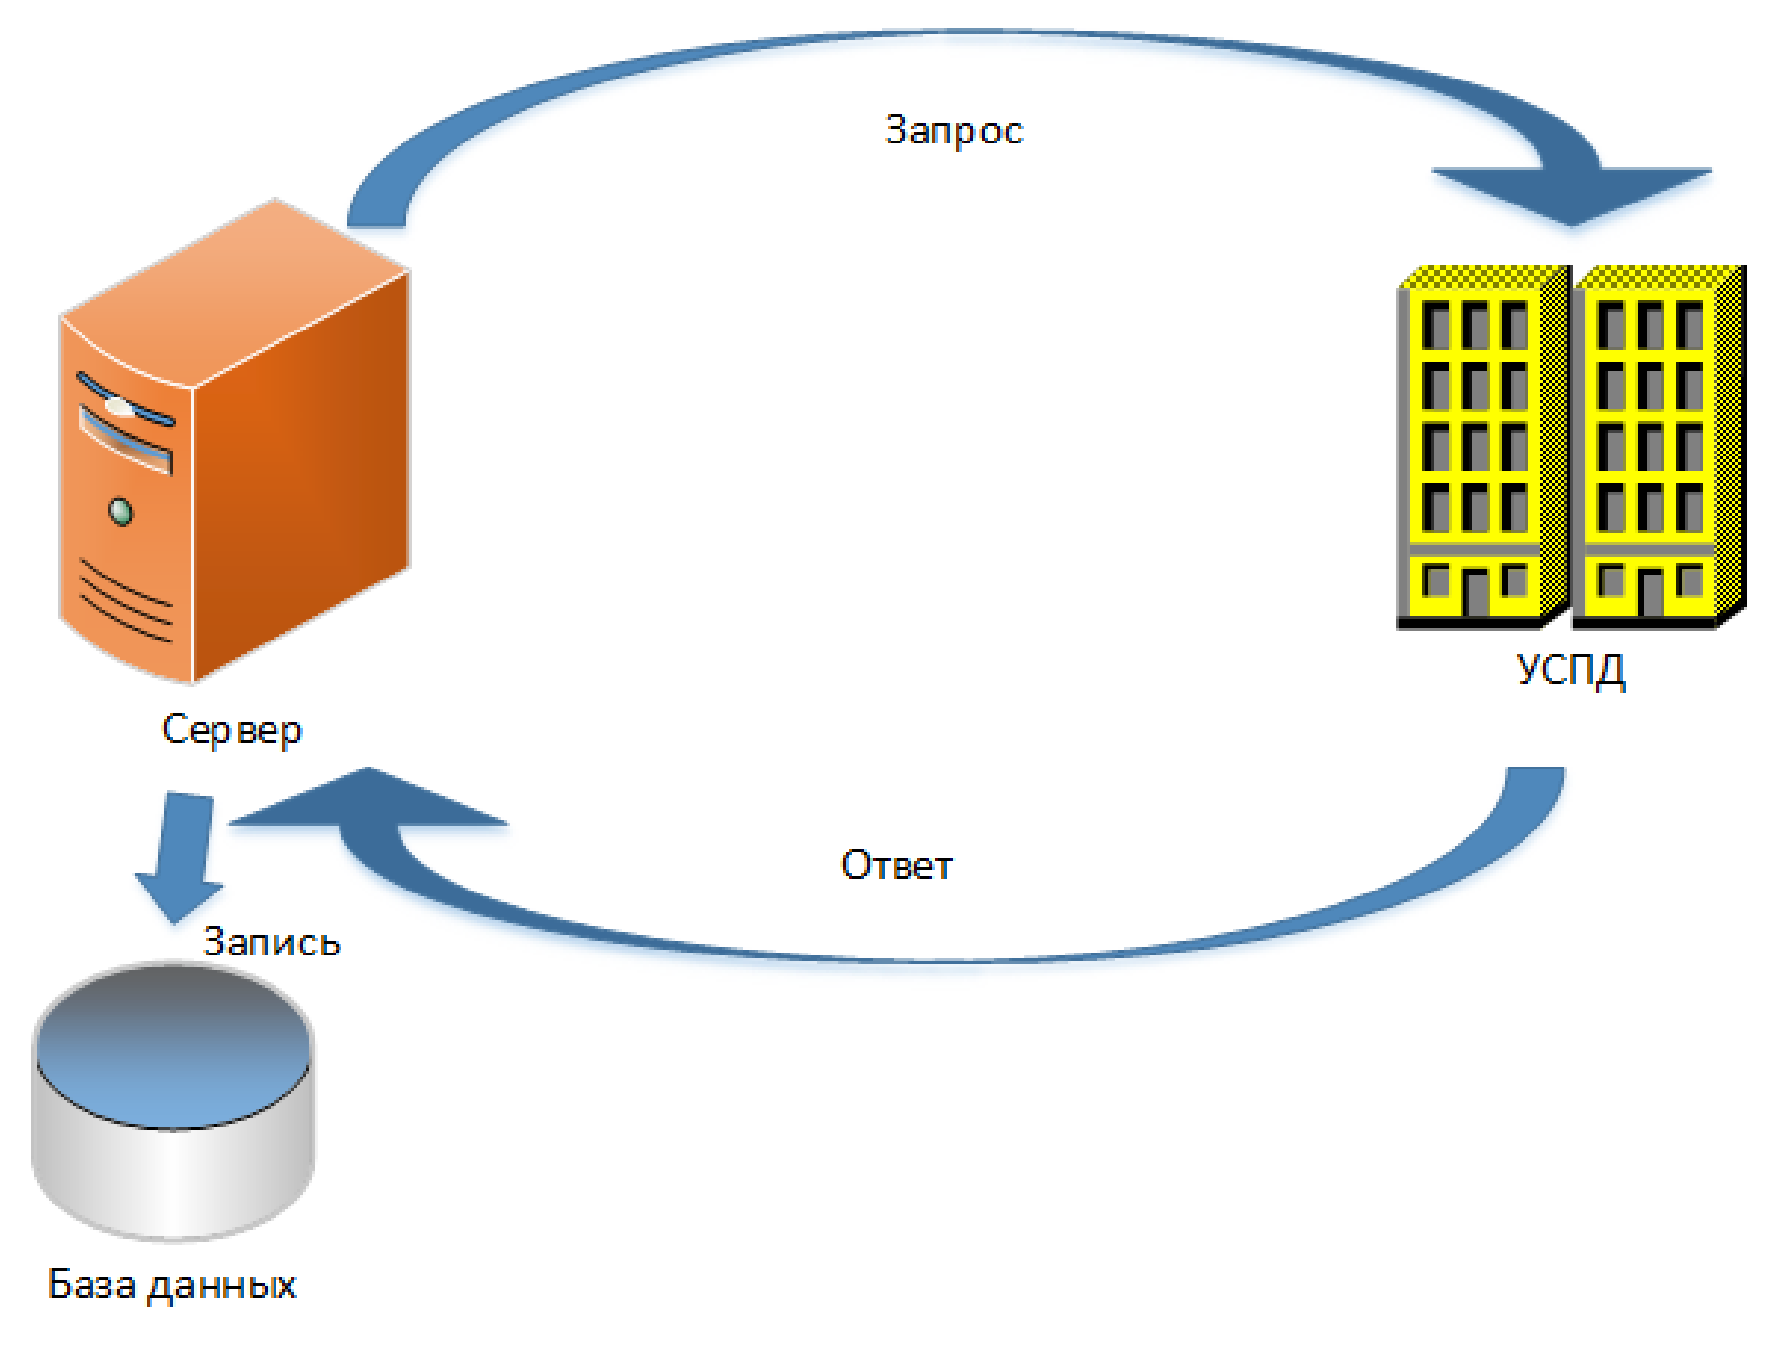
\includegraphics[width=0.8\linewidth]{scheme2}}
 \caption{Схема взаимодействия сервера с УСПД}
 \label{scheme2:scheme2}
\end{figure}

Данный механиз позволяет реализовать опрос УСПД по списку, хранящемуся на сервере, что исключит возможность отправки данных с несанкционированных устройств. Так же появляется возможность обнаружения неисправности УСПД либо ошибки сети, на который сервер будет реагировать предупреждениями. 

Данные, полученные с УСПД, записываются во временную базу данных для последующей обработки и отправки на центральный сервер. В этой же базе данных хранится список всех УСПД, подконтрольных данному серверу. Схема представлена на рисунке \ref{scheme3:scheme3}.

\begin{figure}[!ht]
 \center{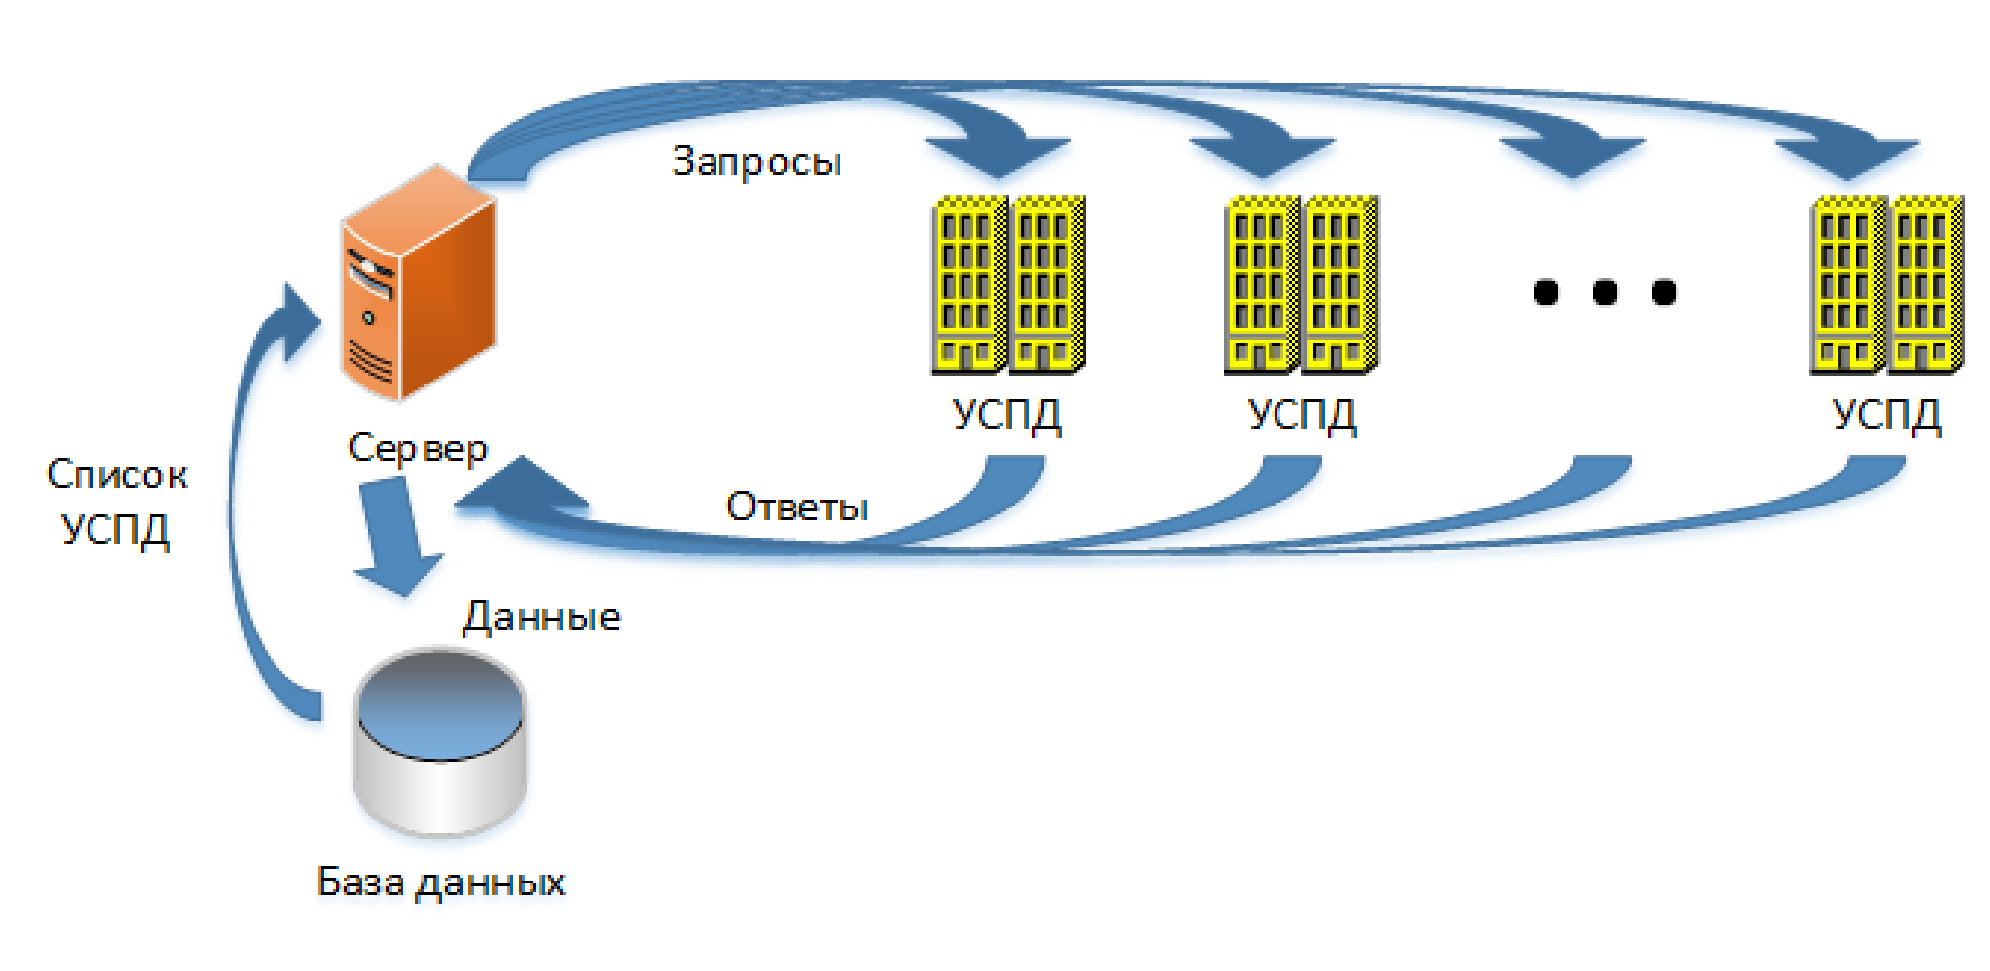
\includegraphics[width=0.8\linewidth]{scheme3}}
 \caption{Механизм взаимодействия с группой УСПД}
 \label{scheme3:scheme3}
\end{figure}

Процедура сбора данных с УСПД осуществляется на основании сформированных оператором правил опроса. Эти правила описывают в какое время и какое УСПД (или группу УСПД) необходимо опросить. В случае отсутствия правил опроса сбор данных производится по стандартной процедуре. Стандартная процедура сбора данных представляет собой последовательный опрос всего списка УСПД, зарегистрированных в системе. Сбор данных с УСПД может проводится в несколько потоков, то есть опрашивать одновременно несколько УСПД. Количество одновременно опрашиваемых УСПД указывается в настройках ССД.
В соответствии с вышеописанными правилами опроса формируются группы УСПД. Для каждой группы УСПД формируется две очереди опроса. Каждая очередь имеет свой временной интервал между опросами, указываемых в настройках ССД. Первая очередь содержит список опрашиваемой группы УСПД, вторая пуста. Из первой очереди происходит опрос УСПД. При успешном обращении к УСПД, оно удаляется из очереди, а в журнал заносится сообщение об успешном проведении операции. Если УСПД не отвечает, то оно переносится во вторую очередь. После опроса всех УСПД из первой очереди начинается опрос второй.
Данная очередь опрашивается несколько раз через небольшие промежутки времени. При ответе УСПД удаляется из очереди, а в журнал заносится сообщение о завершении операции с некоторыми проблемами. Если после последнего цикла опроса во второй очереди останутся УСПД, то о каждом из них в журнал заносится сообщение о неудачном завершении операции получения данных.